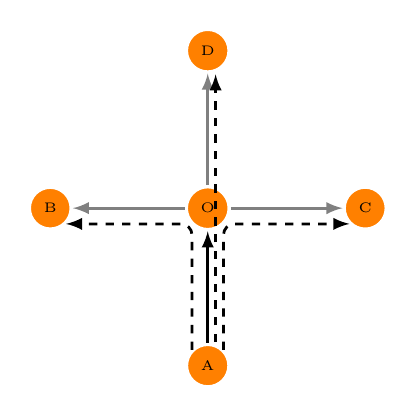
\begin{tikzpicture}[font=\tiny]
    \tikzstyle{node_style} = [draw=white, very thick, circle, fill=orange]
    \tikzstyle{arrow_style1} = [->, black, line width=1, >=latex]
    \tikzstyle{arrow_style2} = [->, gray, line width=1, >=latex]
    \tikzstyle{arrow_style3} = [->, black, line width=3, >=latex]
    \tikzstyle{edge_style2} = [lightgray, line width=1]
    \tikzstyle{line_style1} = [-, gray, line width=1]


    \node[node_style] (n0) at (2,2) {O};
    \node[node_style] (na) at (2,0) {A};
    \node[node_style] (nb) at (0,2) {B};
    \node[node_style] (nc) at (4,2) {C};
    \node[node_style] (nd) at (2,4) {D};

    \draw[arrow_style1] (na) edge (n0);
    \draw[arrow_style2] (n0) edge (nb);
    \draw[arrow_style2] (n0) edge (nc);
    \draw[arrow_style2] (n0) edge (nd);

    \draw[arrow_style1, dashed, rounded corners] (1.8,0.2) -- (1.8, 1.8) -- (0.2, 1.8);
    \draw[arrow_style1, dashed, rounded corners] (2.2,0.2) -- (2.2, 1.8) -- (3.8, 1.8);
    \draw[arrow_style1, dashed] (2.1, 0.3) -- (2.1, 3.7);
\end{tikzpicture}
